\documentclass[a4paper, 12pt, onepage]{article}
\usepackage{graphicx}
\usepackage{lipsum}
\usepackage{mathptmx}

\usepackage{fancyhdr}
\pagestyle{fancy}
\fancyhead{}
\fancyfoot{}
\fancyhead[R]{\thepage\ \hspace{1pt} }

\renewcommand{\headrulewidth}{0pt}
\renewcommand{\footrulewidth}{0pt}

\begin{document}
\pagenumbering{roman}
\addcontentsline{toc}{section}{Title Page}
\begin{titlepage}
  \centering
  
\includegraphics[width=0.2\textwidth]{tu_logo.png}\par
  {\large\scshape Tribhuvan University\par}
  \vspace{0.3cm}
  {\large Pulchowk, Lalitpur \par}
  \vspace{3cm}
  	{\large\scshape A\par}
	{\large\scshape Major Project\par}
        {\large\scshape On\par}
        {\large\scshape Personality Based Music Recommendation System\par}
	\vspace{2.5cm}
        {\large\scshape Submitted by:}\\
        \vspace{0.2cm}
        {
          {\normalsize\verb+Miran Ghimire(070/BCT/521)+}\\
          \vspace{0.1cm}
         {\normalsize\verb+Nabin Bhattarai(070/BCT/522)+}\\
         \vspace{0.1cm}
         {\normalsize\verb+Brihat Ratna Bajracharya(070/BCT/513)+}\\
         \vspace{0.1cm}
        {\normalsize\verb+Abhishek Paudel(070/BCT/502)+}\\
         \vspace{0.1cm}
        }
        \vspace{1cm}
        {\large\scshape Supervised By}\\
        \vspace{0.2cm}
        {
          {\normalsize \verb+Daya Sagar Baral+\par}
          \vspace{0.1cm}
          {\normalsize \verb+Department of+\par}
          \vspace{0.1cm}
          {\normalsize\verb+Electronics and Computer Engineering+}
          \vspace{0.1cm}
        }
\vspace{1cm}
%\\
%{\large\scshape Submitted To}\\
%\vspace{0.2cm}
%{
%  {\normalsize \verb+Naresh Maharjan+\par}
%  \vspace{0.1cm}
%  {\normalsize \verb+Leapfrog Technology+\par}
% }
        \vfill

        % Bottom of the page
	{\normalsize \today\par}
      \end{titlepage}

      \setcounter{page}{2}
      \cleardoublepage
      {
        \setlength{\parskip}{0em}
        \renewcommand\contentsname{Table of Contents}
        \tableofcontents \addcontentsline{toc}{section}{Table of Contents}
      }


      \cleardoublepage
      \pagenumbering{arabic}
      \section{Introduction}
	``\textbf{Personality Based Music Recommendation}'' is the system which uses social media profile of a person to recommend the appropriate music to that user. In this contemporary era of digital technologies, social media has become one of the prominent means for information sharing and communication. Likewise music has been one of the prominent market of entertainment. People listen to music everyday. The fact that music can blend with any emotion has made it's way to different sorts of people with different sorts of personality.\\
	Hence we have come up with the system to recommend the music to a different people based on their social media profiles.Previous work has shown that the information in users social media profiles is reflective of their actual personalities, not an idealized version of themselves, which makes social media platform for studying a people personality.\\
	Several well studied personality models have been proposed, among which the Big Five model is established as the most popular one,which suggests that the regularity in someone's behavior over time and situations uniquely identifies his/her personality type along five dimesions: Openness to experience, Neuroticsm, Extroversion, Aggreableness and Conscientiousness.

      \cleardoublepage
      \section{Summary Of Process}
      \begin{figure}[ht!]
	      \includegraphics[width=450px]{pbrs.png}
		\caption{Block Diagram of a System}
	\end{figure}
	\subsection{Task Analysis}
	\begin{center}
		\begin{tabular}{|c|l|c|c|}
			\hline
				Activity & Description & Immediate Predecessors&Time(weeks)\\
			\hline
			A&Personality DataSet Analysis&-&1\\
			\hline
			B&Feature Extraction from Personality DataSet&A&3\\
			\hline
			C&Personality Analysis Model&B&4\\
			\hline
			D&User Social Media Information Extraction&-&1\\
			\hline
			E&User Personality Analysis&D,C&2\\
			\hline
			F&Music DataSet Analaysis&-&1 \\
			\hline
			G&Feature Extraction from Music DataSet&F&2\\
			\hline
			H&Recommendation Model&G,E&4\\
			\hline
			I&Testing and Debugging&H&2\\
			\hline

		\end{tabular}
	\end{center}
	\cleardoublepage
	\subsection{Task Evaluation}
		\subsubsection{Task Completed}
		\begin{enumerate}
		\item Personality DataSet Analysis
		\item Feature Extraction from Personality DataSet
		\item Personality Analysis Model
		\end{enumerate}

		\subsubsection{Task Remaining}
		\begin{enumerate}
		\item User Social Media Information Extraction
		\item User Personality Analysis
		\item Music DataSet Analysis
		\item Feature Extraction from Music DataSet
		\item Recommendation Model
		\item Testing and Debugging
		\end{enumerate}
      \subsection{Schedule Analysis}
      \begin{figure}[ht!]
	      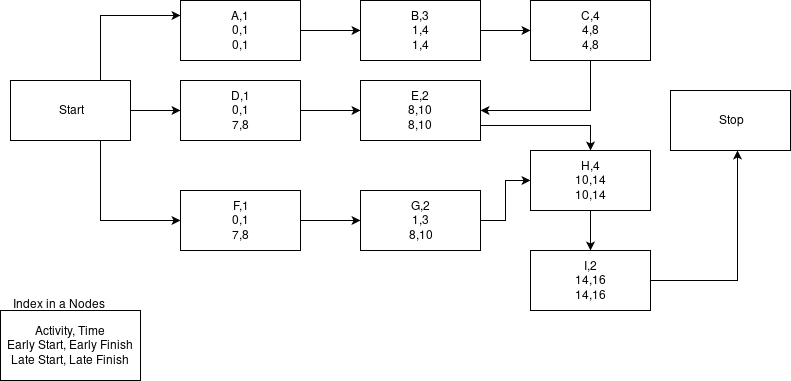
\includegraphics[width=450px]{aschedule.png}
	      \caption{PERT Activity of Node Diagram of Project}
	\end{figure}
	\hfill \break
	Critical path: A-B-C-E-H-I\\
	Estimate time of completion: 16 weeks\\
	Time Elapsed: 4 weeks
	\subsection{Progress Analysis}
	Activity to be completed at this time = A-B-C (4 weeks)\\
	Activity Completed = A-B-C\\
	We are almost within a schedule.
      %\subsection{Budget Analysis}
      %\subsection{Scope Analysis}
      %\subsection{Process Analysis}
      %\subsection{Gantt Progress Chart}

      \section{Activity Analysis}
      \subsection{Task completed till date}
	\begin{center}
		\begin{tabular}{|c|l|c|c|}
			\hline
				Activity & Description & Immediate Predecessors&Time(weeks)\\
			\hline
			A&Personality DataSet Analysis&-&1\\
			\hline
			B&Feature Extraction from Personality DataSet&A&3\\
			\hline
			C&Personality Analysis Model&B&4\\
			\hline
		\end{tabular}
	\end{center}
	\begin{enumerate}
		\item \textbf{Personality DataSet Analysis:}\\
			In order to predict a personality of social media users, myPersonality dataset was used. Dataset was obtained from: 
	\begin{verbatim}
	http://mypersonality.org/wiki/doku.php?id=download_databases 
		\end{verbatim}

		It consisted of:
		\begin{enumerate}
		\item AUTHID : \\ 
			User Id, it was represented with a unique random number in order to protect user's identity.
      \begin{figure}[h!]
	      \centering
	      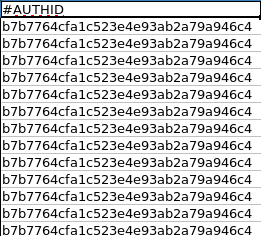
\includegraphics[width=100px]{userid.png}
		\caption{AuthId in dataset}
	\end{figure}
		\item STATUS : \\ 
			It consisted of status posted by the user's in certain time period frame. It consisted of total of 9918 status post of more than 250 users.
      \begin{figure}[h!]
	      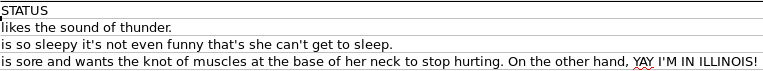
\includegraphics[width=450px]{status.png}
		\caption{status in dataset}
	\end{figure}
		\item PERSONALITY CLASSIFICATION : \\
			It classified personality as Big Five Personality traits which consisted of:\\
		\begin{enumerate}
		\item Openness to Experience:
			curious, intelligent, imaginative. High scorers
			tend to be artistic and sophisticated in taste and appreciate diverse views,
			ideas and experiences.
		\item Conscientiousness:
			responsible, organized, preservering. Conscientious
			individuals are extremely realiable and tend to be high achievers, hard work-
			ers and planners.
		\item Extroverion:
			outgoing, amicable, assertive. Friendly and energetic, ex-
			troverts draw inspiration from social situations.
		\item Agreeableness:
		cooperative, helpful,nurturing. People who score high in
		agreeableness are peace-keepers who are generally optimistic and trusting of
		others.
		\item Neuroticism:
			anxious, insecure, sensitive. Neurotics are moody, tense and
			easily tipped into experiencing negative emotions.
		\end{enumerate}
      \begin{figure}[h!]
	      \centering
	      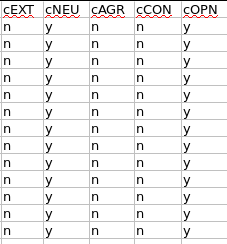
\includegraphics[width=100px]{personality.png}
		\caption{personality classification in dataset}
	\end{figure}
		\end{enumerate}

	\clearpage
	\item Feature Extraction from Personality DataSet:\\
	\begin{enumerate}
	\item Bag of Words:\\
		It is a one of the technique of ``Data Preprocessing'' in NLP in which each word in a document is treated as the feature. It consist of two models:
	\begin{itemize}
		\item Continuous-Gram Model:\\
			It is the model in which every single words that appears in the document is treated as the feature in the sequence in which theyappear. In this model both the presence of the word and appearance sequence both matters.
		\item Skip-Gram Model:\\
			It is the model in which every single words that appears in the document is treated as the feature. However the sequence in which they appear doesn't matter.
	\end{itemize}
	The bag of words model is the most commonly used methods in sentence classification where the frequency of occurence of each word is used as a feture for training a classifier. After the transforming the text into the bag of words, we calculate various measures to characterize the text. The most common type of characteristics calculated from the bag of word is term-frequency i.e the number of times the term appears in the text.\\
	In case, of our project, skip-gram model has been used because the existence of the word in a status posted by the user matters not the sequence in which they appear. After the bag of words extraction, term-frequency has been calculated for the classification purpose.
	\item Stop Words:\\
		It is also one of the technique of ``Data Preprocessing'' in NLP. It is commonly used with bag of words or any kind of models like n-gram in order to elimate the words that are of no use or very less use in the classification purpose. Such as article, preposition etc. The stop word vary within the project to project and depends on specific scenario.\\
		In case of our, project stop words from nltk module has been used. It consist prepostion, article. Besides of the additional stop words also has been added as per the requirement of the project.
	\clearpage
      \begin{figure}[ht!]
	      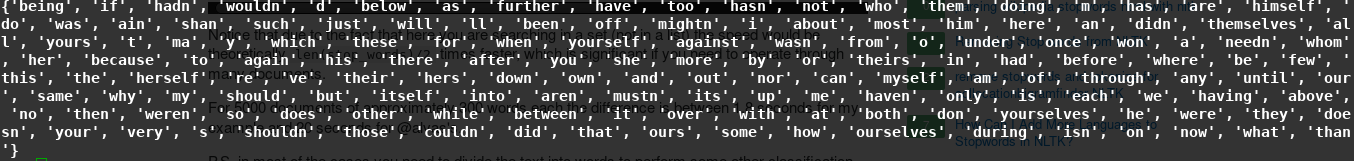
\includegraphics[width=600px]{stopWords.png}
		\caption{stopwords used in the project}
	\end{figure}
	\end{enumerate}
	\item Personality Analysis Model:\\
		For the classification of the personality based on the status update in social media, Naive Bayes Classifier was used.\\
		\textbf{Navie Bayes Classifier:}\\
		It is one of the model used for the classification under the ``Bayesian Classifier''. In machine learning, Naive Bayes classifier are family of simple probabilistic classifiers based on Bayes's theory with assumption of ``independence'' between the features. If the dependence between the features exists Bayesian Network will be used for the classification.
		The major advantage of the Naive Bayes is it's simplicity and highly scalable feature and ability to work easily on huge dataSet. Despite the oversimplified assumptions, Naive Bayes have worked quite well in manycomplex real-world situations.\\
		\textbf	{Problem Formulation:}\\
		Given the set of features $(x_{1},x_{2},x_{3} \ldots x_{n})$
		\\
		Naive Bayes classifies into a class $c$ as:\\
		$p(C_{k}|x) = argmax \frac{(p(C_{k}) * p(x|C_{k})} { p(x)} $\\

		where, $p(C_{k})$ is known as prior probability
		\\ and, $(p(x|C_{k})$ is known as prosterior probability
		In practise, there is interest only in the numerator of that fraction, because the denominator does not depend on C and the values of the features for a given set of features are constant, so the denominator is effectively constant, hence inorder to maximize the function denominator is ignored and the model becomes:
\\
\begin{equation}
		p(C_{k}|x) = {(p(C_{k}) * p(x|C_{k})}  \\
\end{equation}
	which can also be written as:
	$p(C_{k}|x) = prior probability * prosterior probability$
	For a classification of sentence or document ``Mutinominal Naive Bayes'' is one of the popular model which has been used in the project. With a mulinominal model, features represent the frequencies with which certain events have been generated by multinominal i.e feature set.
	\\
	\textbf{Additive Smooting:} \\
	In statistics, additive smoothing, also called Laplace smoothing, is a technique used to smooth categorial data. Given a oberservation $x = (x_{1},x_{2},\cdots,x_{n})$ from a multinominal distribution with N trials and parameter vector $\theta = (\theta_{1},\ldots,\theta_{d})$ smoothed version o the data gives the estimator:\\
	$\theta = \frac{x_{i} + \alpha}{N+\alpha *d}$ \\
	when $\alpha = 1 $, it's called add one Laplace smoothing which has been used as the smoothing technique in the project.
	Overfitting : \\
	In order to reduce the overfitting of the classifier, $k^{th}$-fold cross validation technique is used. The advantage of this method is that all observations are used for both training and validation, and each observation is used for validation exactly once.\\
	In the project, $5^{th}$-fold cross validation technique is applied in which the data set is divided into the 5 test cases and train cases and classifier is trained on each of those cases.
	\\
	\textbf{Underfitting :}\\
	Underfitting in the Naive Bayes classifier, can occur whenever the probabilities: prior or prosterior are very small, in this case in order prevent the program from underfitting, resulting from the multiplication of the very small terms, $\log$ can be used after which the resulting equation becomes:\\
	$p(C|x) = \log p(C) + \sum_{i=1}^{k} \log(x|C) $
	\\
	\textbf{Optimization: }\\
	Classifier Naive Bayes, as seen from the above equation, classifies feature set into a class via the multiplication of the prior and posterior probability which requires their computation each time the classifier tires to classify the feature set into class. \\
	In order to solve the above problem, posterior probability is precomputated and stored on \textbf{HashTable}, where it's stores the posterior probability of each feature set, which can be easily be retrieved and used for the classification in the program.
      \begin{figure}[h!]
	      \centering
	      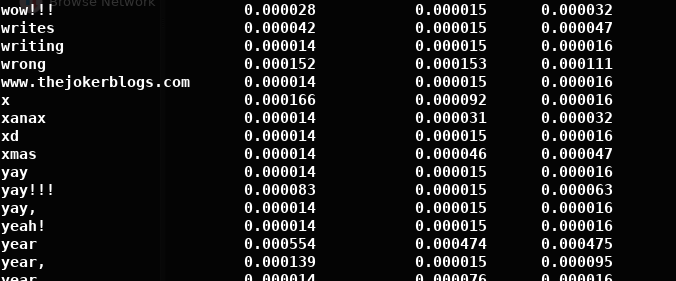
\includegraphics[width=200px]{hashtable.png}
	      \caption{sample of hashtable of a project}
	\end{figure}
	\end{enumerate}
	\subsection{Current Deliverable}
	\begin{itemize}
	\item Personality Prediction Model:
		It predict's the personality of the user based on the status of the user.
	\end{itemize}
\subsection{Output}
      \begin{figure}[h!]
	      \centering
	      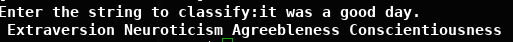
\includegraphics[width=200px]{output.png}
	      \caption{sample of output of a project}
	\end{figure}
	\subsection{Accuracy}
	\subsubsection{Overfitting}
	In order to remove the overfitting of data set into the real world application $k^{th}$ fold cross validation technique was used. \\
	Within our program $5^{th}$ fold cross validation technique was used under which data set was divided into train set and test set 5 times in which first train and test set consisted of first 80\% and 20\% of data and second consisted of second 80\% and 20\% respectively and so on.
      \begin{figure}[h!]
	      \centering
	      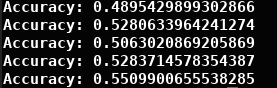
\includegraphics[width=200px]{accuracy.png}
	      \caption{Accuracy of classifier in 5th fold cross validation}
	\end{figure}
    %  \subsection{Short term future tasks and deliverable}

    %  \cleardoublepage
    % \section{Previous problems and issues}
    %  \subsection{Action item and status} %k vanya maile bujhena hai
    %  \subsection{New or revised action items} %yo ni

      \cleardoublepage
      \section{Current problems and issues}
      After training  the classifier the accuracy of the classifier was not so satisfactory.
      \subsection{Problems}
      \begin{itemize}
	\item Problem might have been on feature extraction where the bag of words model was used.
	\item Problem also could be the limited scope of the stop words in the feature extraction.
	\end{itemize}
      \subsection{Issues}
      \begin{itemize}
      \item Training takes time i.e a bit time consuming
	\item Accuracy of the classifier is not satisfactory.
	\end{itemize}
      \subsection{Possible solutions}
      \begin{itemize}
	\item Stop Words scope can be increased via the introduction of the additional stop words.
	\item If accuracy problem persists even after increasing the stop words, feature extraction model can be upgraded into the n-gram model.
	\item Training time can be reduced with the help of the optimization again where boradening the scope of the stop words can be very useful.
	\end{itemize}
  %    \subsubsection{Recommendation}
  %    \subsubsection{Assignment of responsibility}
  %    \subsubsection{Deadline}
      \clearpage
      \section{Task to be completed in Future}
	\begin{center}
		\begin{tabular}{|c|l|c|c|}
			\hline
				Activity & Description & Immediate Predecessors&Time(weeks)\\
			\hline
			D&User Social Media Information Extraction&-&1\\
			\hline
			E&User Personality Analysis&D,C&2\\
			\hline
			F&Music DataSet Analaysis&-&1 \\
			\hline
			G&Feature Extraction from Music DataSet&F&2\\
			\hline
			H&Recommendation Model&G,E&4\\
			\hline
			I&Testing and Debugging&H&2\\
			\hline
		\end{tabular}
	\end{center}
\end{document}

%%% Local Variables:
%%% mode: latex
%%% TeX-master: t
%%% End:
